%%%%%%%%%%%%%%%%%%% CONFIGURAZIONE
\documentclass[11pt,oneside,a4paper,italian]{article}
%\usepackage[scale = 0.75]{geometry}
\usepackage[left=3cm,top=3cm,right=3cm,bottom=3cm]{geometry}
%\usepackage[a4paper]{geometry}
\usepackage{sectsty}
\usepackage[adobe-utopia]{mathdesign}
\usepackage{helvet}
%\usepackage{amsmath,amssymb,amsfonts,textcomp}
\usepackage{calc}
\usepackage{amsmath}
\usepackage[latin1]{inputenc}
\usepackage[OT2,T1]{fontenc}
\usepackage[italian]{babel}
\usepackage[pdftex]{graphicx,color}
\graphicspath{{img/}}
\DeclareGraphicsExtensions{.pdf}
\usepackage{subfigure}
\usepackage[hyperindex]{hyperref}
\usepackage[figure,table]{hypcap}
\usepackage[hang, small, bf, margin=20pt, tableposition=top]{caption}
\definecolor{gray}{rgb}{.200,.250,.250}
\hypersetup{colorlinks=true, linkcolor=gray, urlcolor=gray, anchorcolor = gray, citecolor = gray, filecolor = gray, urlcolor = gray, pdftitle={SCAF : Power Detector}, pdfsubject = {ISM 2.4GHz Band Power Detector}, pdfkeywords = {matching, CAD, AWR, microwave, office, power, detector, ISM, 2.4}, pdfauthor = {Stefano Diamante, Alberto Landini, Laurent Ntibarikure} , pdfcenterwindow=true, pdfdisplaydoctitle=true, pdfstartview=FitH, pdfcreator={}, bookmarksopen=true, bookmarksopenlevel=\maxdimen, CJKbookmarks=true, pdfpagemode=UseOutlines, colorlinks=true, linktocpage=true,citecolor={blue}} % pdfpagemode=UseOutlines for bookmarks UseNone for nothing
%\pagestyle{empty}
%%%%%%%%%%%%%%%%%%%%%%%%%%%%%%%%%%%%%%%%%%%%%%%%%%%%%%%%%%%%%%%%%%%%%%%%%%%%%%%%
% DOCUMENTO
%%%%%%%%%%%%%%%%%%%%%%%%%%%%%%%%%%%%%%%%%%%%%%%%%%%%%%%%%%%%%%%%%%%%%%%%%%%%%%%%
\begin{document}

\clearpage
\selectlanguage{italian}
\title{\textsc{\textbf{\Huge{Progetto di un Rivelatore di Potenza \\ con Diodo HSMS2850}}}}
\author{Stefano Diamante, Gabriele Giannini, Laurent Ntibarikure}
\date{Marzo 2009}
\maketitle

\begin{abstract}
Si presentano le fasi di progetto di un rivelatore di potenza operante in banda ISM 2.4 GHz. Le simulazioni vengono eseguite con il software Microwave Office dell'AWR, permettendo di prevedere accuratamente il comportamento del circuito progettato.
\end{abstract}

\tableofcontents
\pagestyle{plain}
\newpage
%%%%%%%%%%%%%%%%%%%%%%%%%%%%%%%%%%%%%%%%%%%%%%%%%%%%%%%%%%%%%%%%%%%%%%%%%%%%%%%% 
\section{Introduzione}

\par I rivelatori di potenza sono dispositivi di largo impiego nell'ambito delle telecomunicazioni wireless. Questi permettono di rilevare la potenza di un segnale a radiofrequenze (RF) in modo da adattare, per esempio, la catena di ricezione alla potenza di segnale ricevuto. In effetti, il guadagno degli amplificatori a monte della catena di ricezione viene controllato in funzione della potenza ricevuta.

\par Lo schema del rivelatore di potenza � illustrato nella seguente figura \ref{fig:RivSchem}.
\begin{figure}[ht!]
\centering
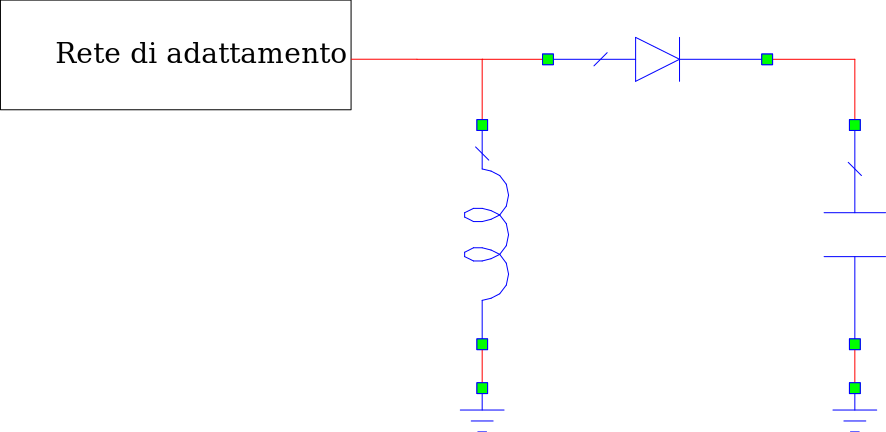
\includegraphics[scale=0.4]{SchemaRivelatore}
\caption{Schema circuitale del rivelatore di picco.}
\label{fig:RivSchem}
\end{figure}
\par La rivelazione si basa sulla conversione, per le non linearit� del diodo,  della potenza del segnale RF incidente sull'anodo del diodo in una componente continua (DC) sul condensatore collegato al catodo. L'entit� di potenza trasferita in continua invece che alle armoniche superiori determina la sensibilit� del rivelatore di potenza. Quest'ultima dipende dalle caratteristiche intrinseche del diodo. Il diodo che verr� utilizzato � l'HSMS2850 dell'Agilent. Trattasi di un diodo Schottky ``Zero Bias'', ovvero un diodo che non necessita di rete di polarizzazione, la tensione di soglia essendo nulla. Il produttore ne consiglia l'impiego per rilevare potenze al disotto di qualche {$\mu$}W (sotto i -20 dBm \cite{HSMS2850DataSheet}), range di potenze in cui la caratteristica di trasferimento (da potenza RF a tensione DC) del rivelatore � pressoch� lineare.

\section{Adattamento}

\par Il circuito del rivelatore richiede una rete di adattamento ai fini di massimizzare il trasferimento di potenza ($\mathrm{Z_{IN} = Z_{OUT}^{*}}$) ed allo stesso tempo minimizzare le riflessioni ($\mathrm{Z_{IN} = Z_{OUT}}$ tale che $\mathrm{\Gamma = 0}$) sul diodo. Entrambe le condizioni si ottengono trasformando ad un valore puramente resistivo ($\mathrm{Z_{IN}}$ e $\mathrm{Z_{OUT}}$ reali) le impedenze di uscita per il circuito a monte e quella d'ingresso per il circuito a valle. Per convenzione, nei circuiti RF odierni viene utilizzato il valore di 50 $\Omega$.
\par Vi sono diverse tecniche di adattamento di impedenza : le reti a L, che impiegano componenti concentrati reattivi, gli stubs ed il trasformatore a $\lambda$/4, entrambi costituiti da tratti di linea di trasmissione opportunamente collegati. Verranno presentati due tipi di reti a L, con induttanza e capacit�, ed un adattamento a singolo stub in microstriscie di 50 $\Omega$.

\subsection{Circuito Lineare del Diodo}

\par Il diodo HSMS2850 pu� essere approssimato col circuito a costanti concentrate fornito dal produttore \cite{HSMS2850DataSheet}, illustrato in figura \ref{fig:CircLineareDiodoProduttore} dove $\mathrm{L_P}$ e $\mathrm{C_P}$ corrispondo all'induttanza serie e la capacit� parallela parassite del package SOT23.
\begin{figure}[ht!]
\begin{minipage}[b]{0.5\linewidth} % A minipage that covers half the page
\centering
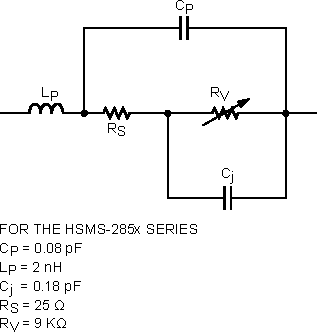
\includegraphics[width=7cm]{EqCirc_HSMS2850}
\caption{Modello equivalente del diodo fornito dal costruttore.}
\label{fig:CircLineareDiodoProduttore}
\end{minipage}
\begin{minipage}[b]{0.5\linewidth}
\centering
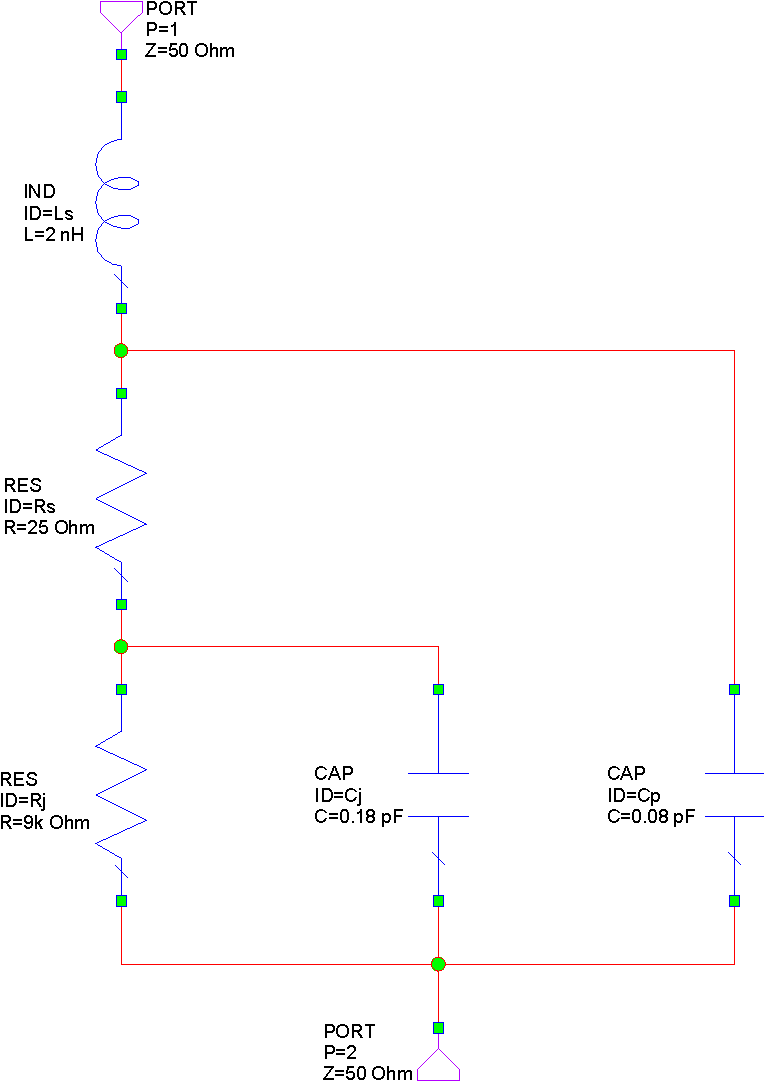
\includegraphics[width=7cm]{LinearDiode}
\caption{Circuito \textsf{``LinearDiode''} ricostruito in Microwave Office per l'analisi di scattering.}
\label{fig:MWOfficeLinearDiode}
\end{minipage}
\end{figure} Tale circuito � stato costruito in Microwave Office come illustrato in figura \ref{fig:MWOfficeLinearDiode} per proseguire con la simulazione dei parametri di scattering, valutati rispetto ad una porta di 50 $\Omega$ come si pu� vedere in figura \ref{fig:ZinDiodo}.
\begin{figure}[ht!]
\centering
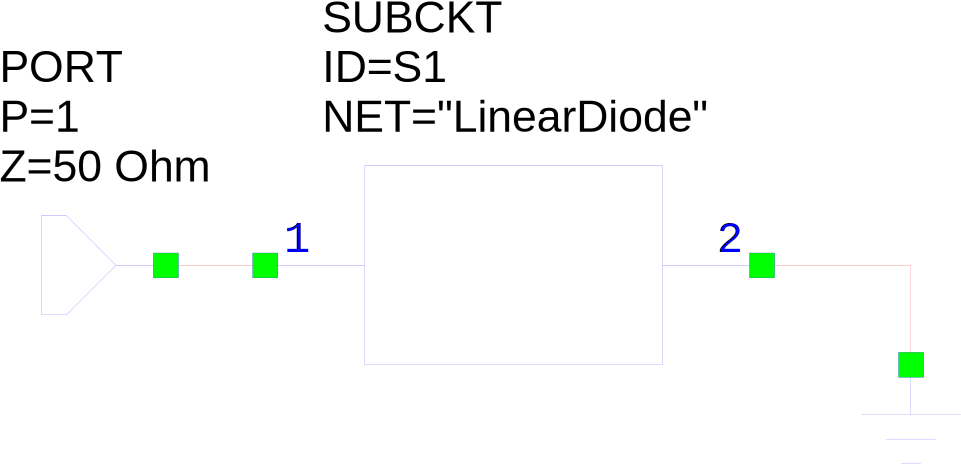
\includegraphics[scale=0.3]{ZinDiodo}
\caption{Valutazione dell'impedenza d'ingresso del diodo.}
\label{fig:ZinDiodo}
\end{figure} L'impedenza d'ingresso $\mathrm{Z_{IN}}$ del diodo a 2,45 GHz � di circa $18,9 + j 219,4$ $\Omega$. In seguito vengono presentate le reti di adattamento scelte tali da riportare, a 2,45 GHz, la $\mathrm{Z_{IN}}$ a 50 $\Omega$.

\subsubsection{Adattamento con Rete a L : L serie e C parallelo}\label{par:LsCp}

\par Il primo adattamento realizzato � una rete a L con induttanza serie, tale da portare il carico ohmico-capacitivo del diodo ad una impedenza ohmico-induttiva di conduttanza 0,02 S (muovendosi sul cerchio ad resistenza costante 18,9 $\Omega$ della carta di Smith), e una capacit� parallela che porti infine (muovendosi sul cerchio a conduttanza costante 0,02 S) l'impedenza complessiva al valore puramente resistivo di 50 $\Omega$. I valori di induttanza e capacit� sono stati individuati sfruttando l'opzione di 
``tuning'' che offre il software, che permette di variare gradualmente con una barra a scorrimento tali parametri come si pu� vedere in figura \ref{fig:LinearPD_LC_1}, velocizzando cos� la procedura di adattamento. Lo scorrimento implica, in tempo reale, uno spostamento del carico sulla carta di Smith e la sua traiettoria, per la rete di adattamento utilizzata, � quella illustrata in figura \ref{fig:LCMatchingProcedure}.
\begin{figure}[ht!]
\centering
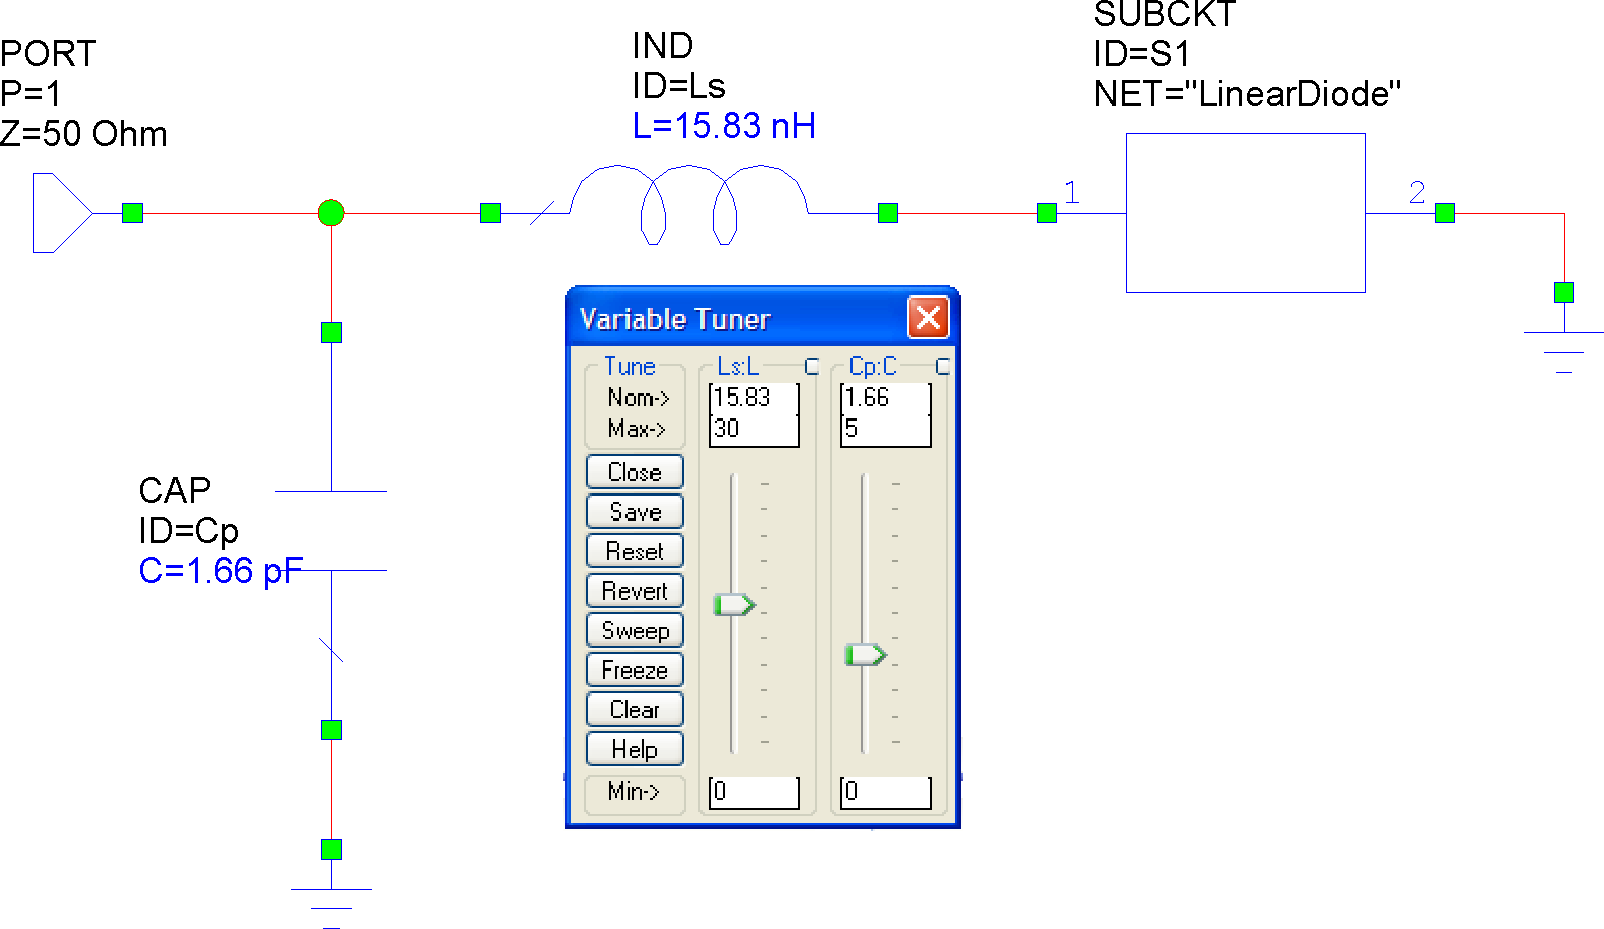
\includegraphics[scale=0.5]{LinearPD_LC_1}
\caption{Rete di adattamento $\mathrm{L_S}$/$\mathrm{C_P}$ e finestra di tuning.}
\label{fig:LinearPD_LC_1}
\end{figure}
\begin{figure}[ht!]
\centering
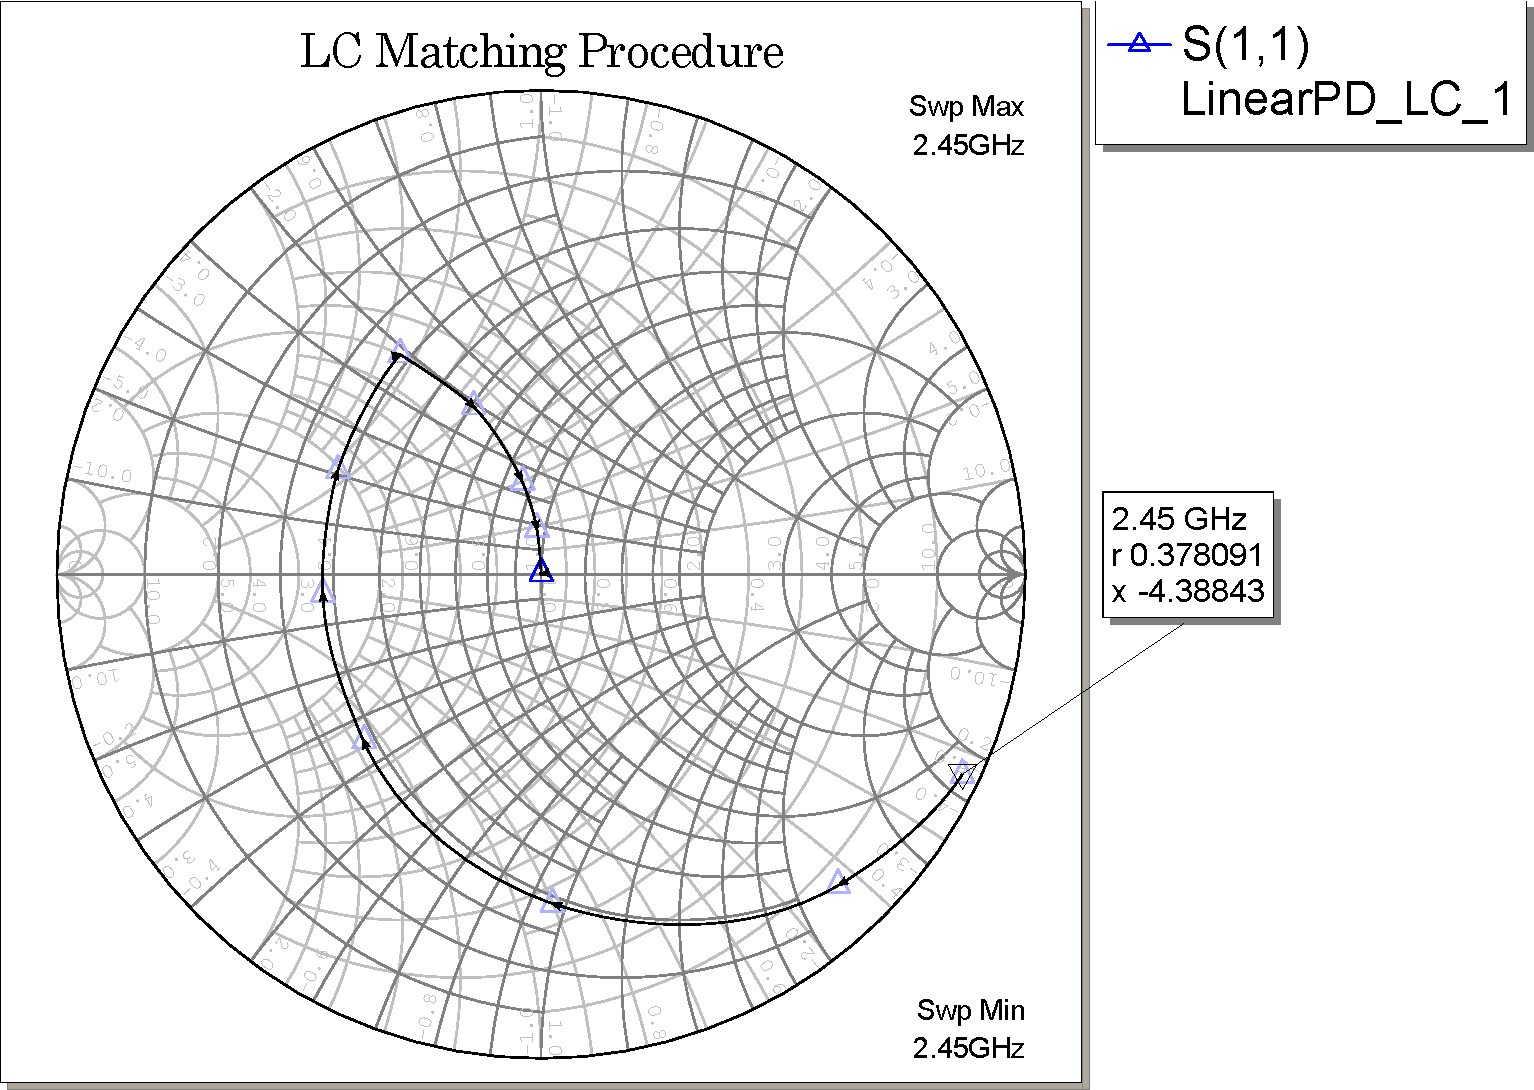
\includegraphics[scale=0.5]{LCMatchingProcedure}
\caption{Traiettoria sulla carta di Smith del carico costituito dal diodo a fronte di variazioni delle induttanze e capacit� della rete a L.}
\label{fig:LCMatchingProcedure}
\end{figure} I valori ottenuti sono di 15,83 nH per l'induttanza serie e 1,66 pF per la capacit� parallela.

\subsubsection{Adattamento con Rete a L : L parallelo e C serie}

\par La procedura di adattamento in questo caso � simile a quella presentata nel precedente paragrafo \ref{par:LsCp}. Varia leggermente la traiettoria in quanto ci si sposta inizialmente su un cerchio a conduttanza costante ed infine su quello ad resistenza costante 50 $\Omega$. Il circuito cos� realizzato � quello presentato in figura \ref{fig:LinearPD_LC_2}.
\begin{figure}[ht!]
\centering
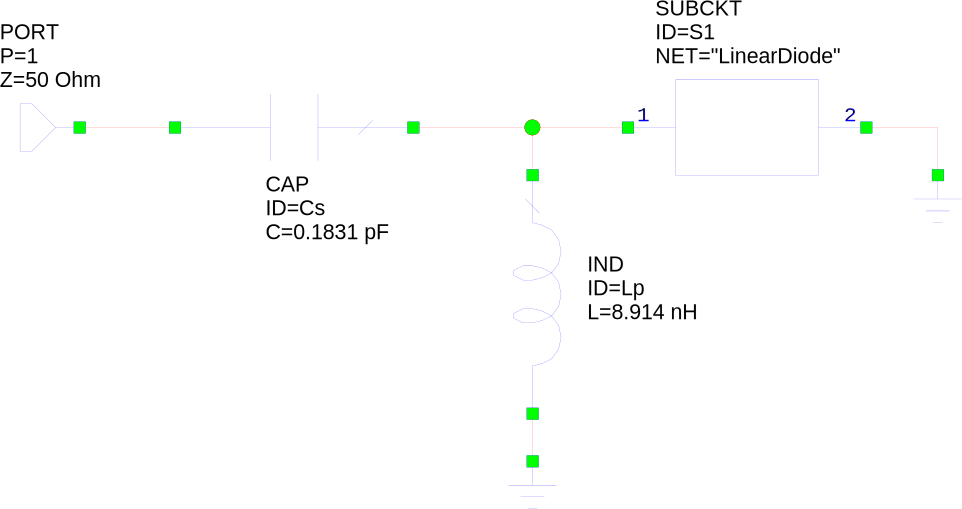
\includegraphics[scale=0.5]{LinearPD_LC_2}
\caption{Rete di adattamento $\mathrm{L_P}$/$\mathrm{C_S}$.}
\label{fig:LinearPD_LC_2}
\end{figure} I valori ottenuti sono circa di 8,9 nH per l'induttanza parallela e 0,18 pF per la capacit� serie.

\subsubsection{Adattamento a Singolo Stub in microstriscia}

\par

\begin{figure}[ht!]
\centering
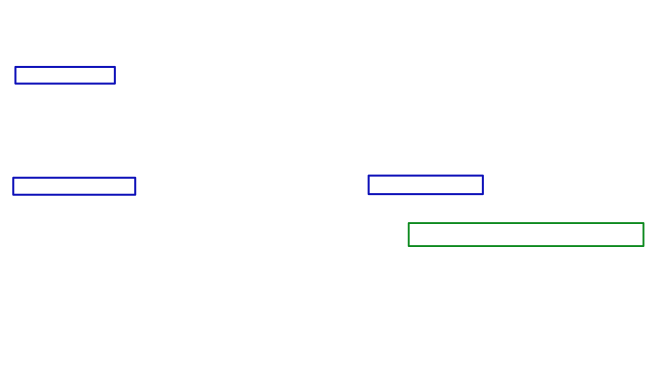
\includegraphics[scale=0.8]{TxLineTool}
\caption{Tool di calcolo della geometria della microstriscia di 50 $\Omega$.}
\label{fig:TxLineTool}
\end{figure}


\begin{figure}[ht!]
\centering
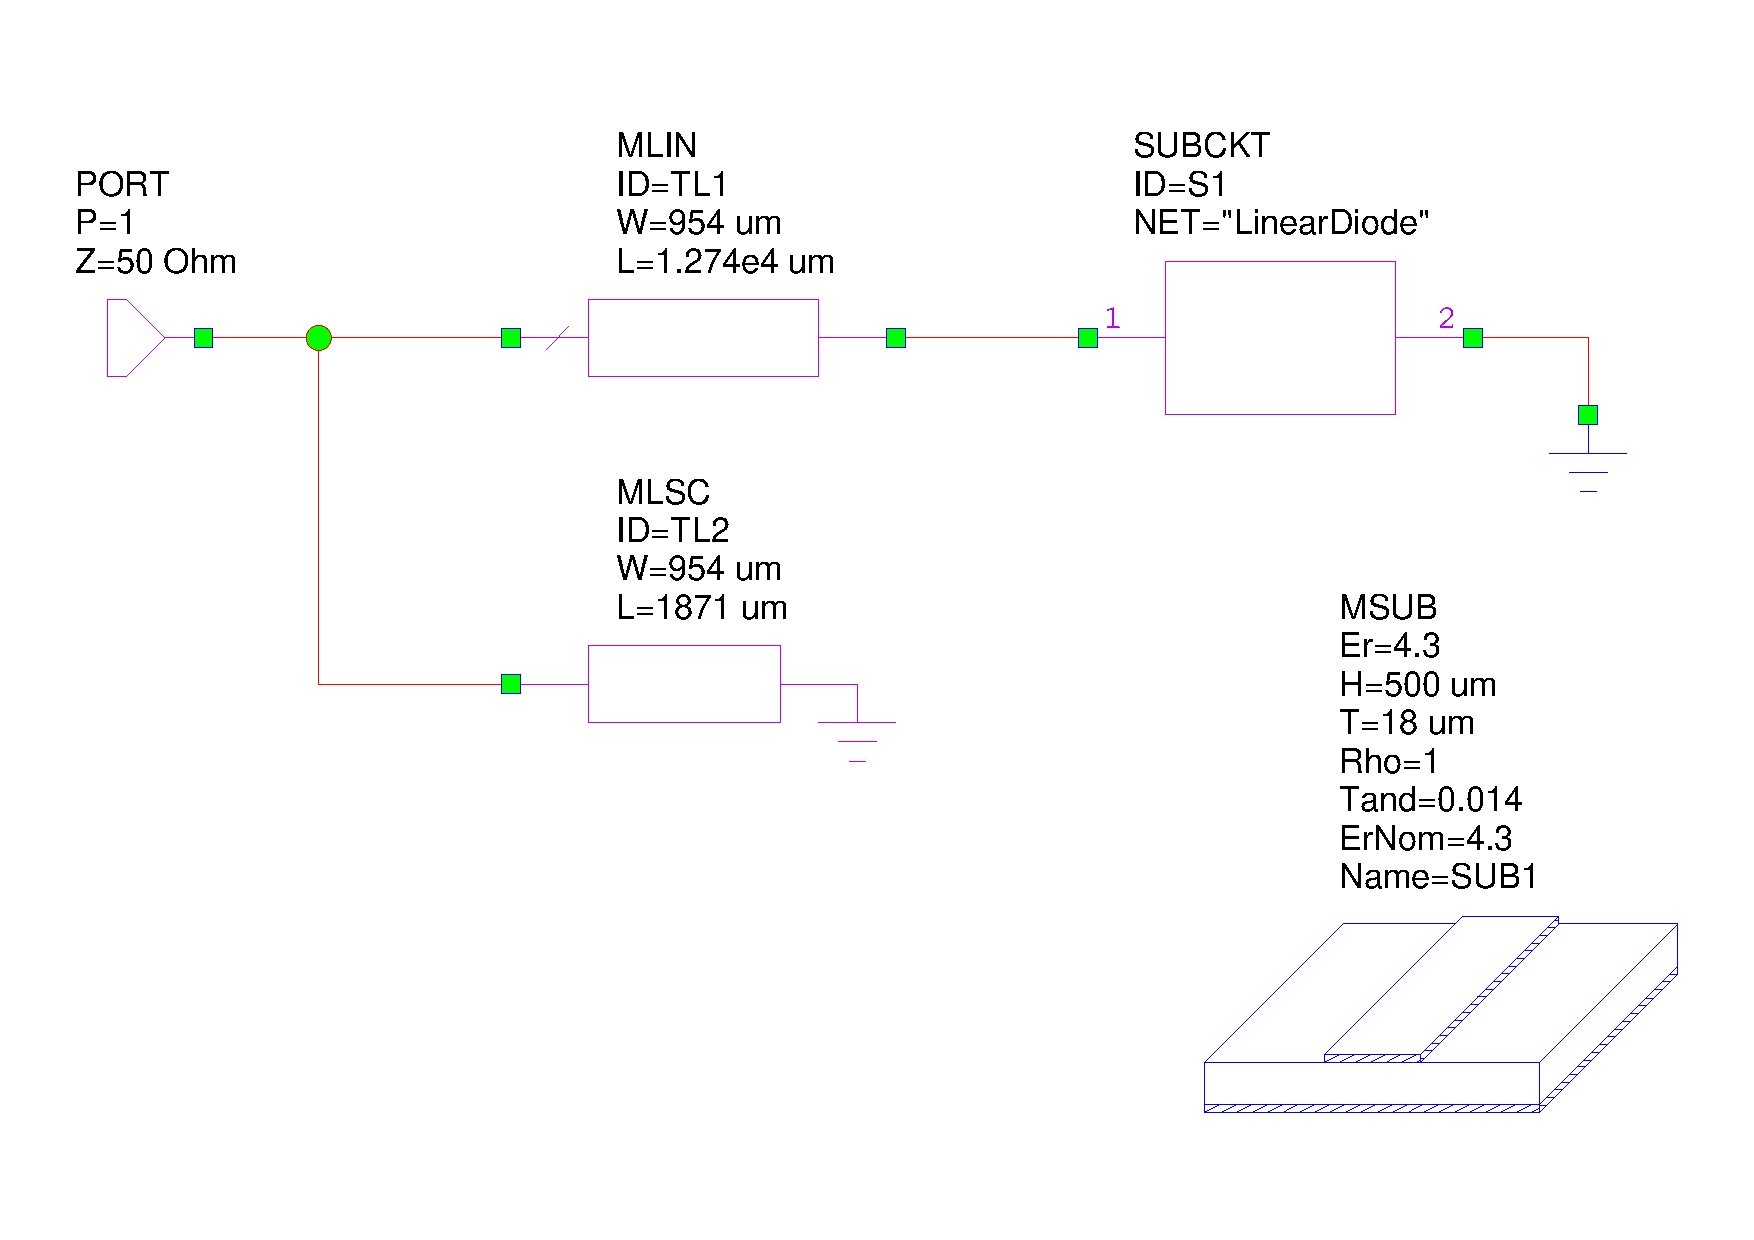
\includegraphics[scale=0.5]{LinearPD_uStrip}
\caption{Rete di adattamento a stub in microstriscia di 50 $\Omega$.}
\label{fig:LinearPD_uStrip}
\end{figure}

\section{Conclusione}

\begin{thebibliography}{9}

\bibitem{HSMS2850DataSheet} Agilent Tecnologies, Technical Data, \emph{HSMS-2850 Series}.

\end{thebibliography}

\end{document}
